\chapter*{\FontH{\Huge Tabea Timpetampe und Herr Häusler}}
\addcontentsline{toc}{chapter}{Tabea Timpetampe und Herr Häusler}
\lettrine[lines=3]{\color{DeepPink}T}{abea} Timpetampe sitzt im Sandkasten und spielt. Sie hat gerade ein Dach auf ihr Sandhaus gebaut, als ihr einfällt, dass das Dach ja auch nass werden kann, wenn es regnet. Also baut sie noch ein Dach für das Dach. Und für dieses dann auch noch eins und noch eins und noch eins oben drauf.

\enquote{Was machst Du da?} Eine Weinbergschnecke ist auf Tabea Timpetampes Eimerchen geklettert und bestaunt das Bauwerk. 

\enquote{Ich baue eine Burg}, antwortet Tabea Timpetampe, denn sie bemerkt gerade, dass das Dach auf dem Dach eines Daches viel mehr wie ein Turm aussieht. Und Türme gehören zu Burgen. Aber wenn sie schon einmal Besuch hat, kann sie ja eigentlich auch gleich mal eine Pause machen. In einem Döschen hat sie noch Banane von Mama bekommen, die gerade dabei ist, mit ihrer grossen Schwester Fahrradfahren zu üben. 

Die Banane in Stücke zu schneiden ist ja wohl das Dümmste, das kann sie heute gar nicht leiden. Ein Glück, dass Tabea Timpetampe die beste Köchin des Sandkasten ist. Im Nu hat sie eine herrliche Suppe aus Sand und Gras und Blumen gezaubert. Rein mit der Banane und abschmecken. Prima, die knirscht wenigstens zwischen den Zähnen, da kann man auch gleich hören, ob man isst, falls man mal gerade keine Lust hat, zu schmecken.

\enquote{Wenn ich mal gross bin, dürfen meine Kinder immer nur Banane mit Suppe essen.}, erklärt sie der Schnecke. Die streckt nur ihre Fühler gelangweilt in Richtung Sonne. Die Schnecke ist schon alt, schon fast ein Jahr und wenn man so alt ist, mag man den Satz \textit{Wenn ich mal gross bin, dürfen meine Kinder \dots} einfach nicht mehr hören.

\enquote{Ich muss weiter}, erklärt die Schnecke, \enquote{Ich jogge gerade und da darf man nicht kalt werden. Immer in Bewegung bleiben, sonst werden die Muskeln hart.} Und mit einem \textit{Hopp, Hopp, Hopp} joggt sie  davon.

Tabea Timpetampe staunt überhaupt nicht, dass Schnecken joggen. Was sollen die denn sonst für eine Sportart treiben, bitteschön? Ohne Arme kann man kein Federball spielen und ohne Füsse kein Fussball. Da bleibt nur noch das Joggen übrig. 

Sport sei gesund, behauptet Papa. Das behauptet er auch bei Brokkoli und wenn er das Fenster öffnet, obwohl es kalt draussen ist und wenn sie ins Bett soll, obwohl sie noch gar nicht schlafen will. Gesund muss also irgendetwas schlechtes bedeuten, schlussfolgert Tabea Timpetampe nicht ganz richtig, denn Papas haben gewöhnlich immer Recht. Also lieber schnell die Schnecke retten, bevor noch etwas Schlimmes passiert.

Zum Glück ist die Schnecke noch nicht sehr weit gekommen mit ihrem Joggen, gerade will sie nach dem Schäufelchen seitlich abbiegen, da wird sie von Tabea Timpetampe hoch gehoben und auf den Rand des Sandkastens gesetzt -- zur Rettung. 

\enquote{Liebe Frau Schnecke}, fängt sie an zu erklären, wird aber unterbrochen.

\enquote{Ich bin ein Herr und keine Frau und wenn es dir nicht zu viele Umstände macht, ich heisse Herr Häusler. Wir Weinbergschnecken haben ein Häuschen auf dem Rücken und heissen deswegen alle Häusler. Das ist eine Stilfrage. Jedenfalls will ich mit unbehausten Schnecken nicht verwechselt werden. Das nennt man Kultur, das wirst du schon noch lernen, junge Dame.}

\afterpage{
    \begin{figure}
        \thispagestyle{empty}    
        \centering
        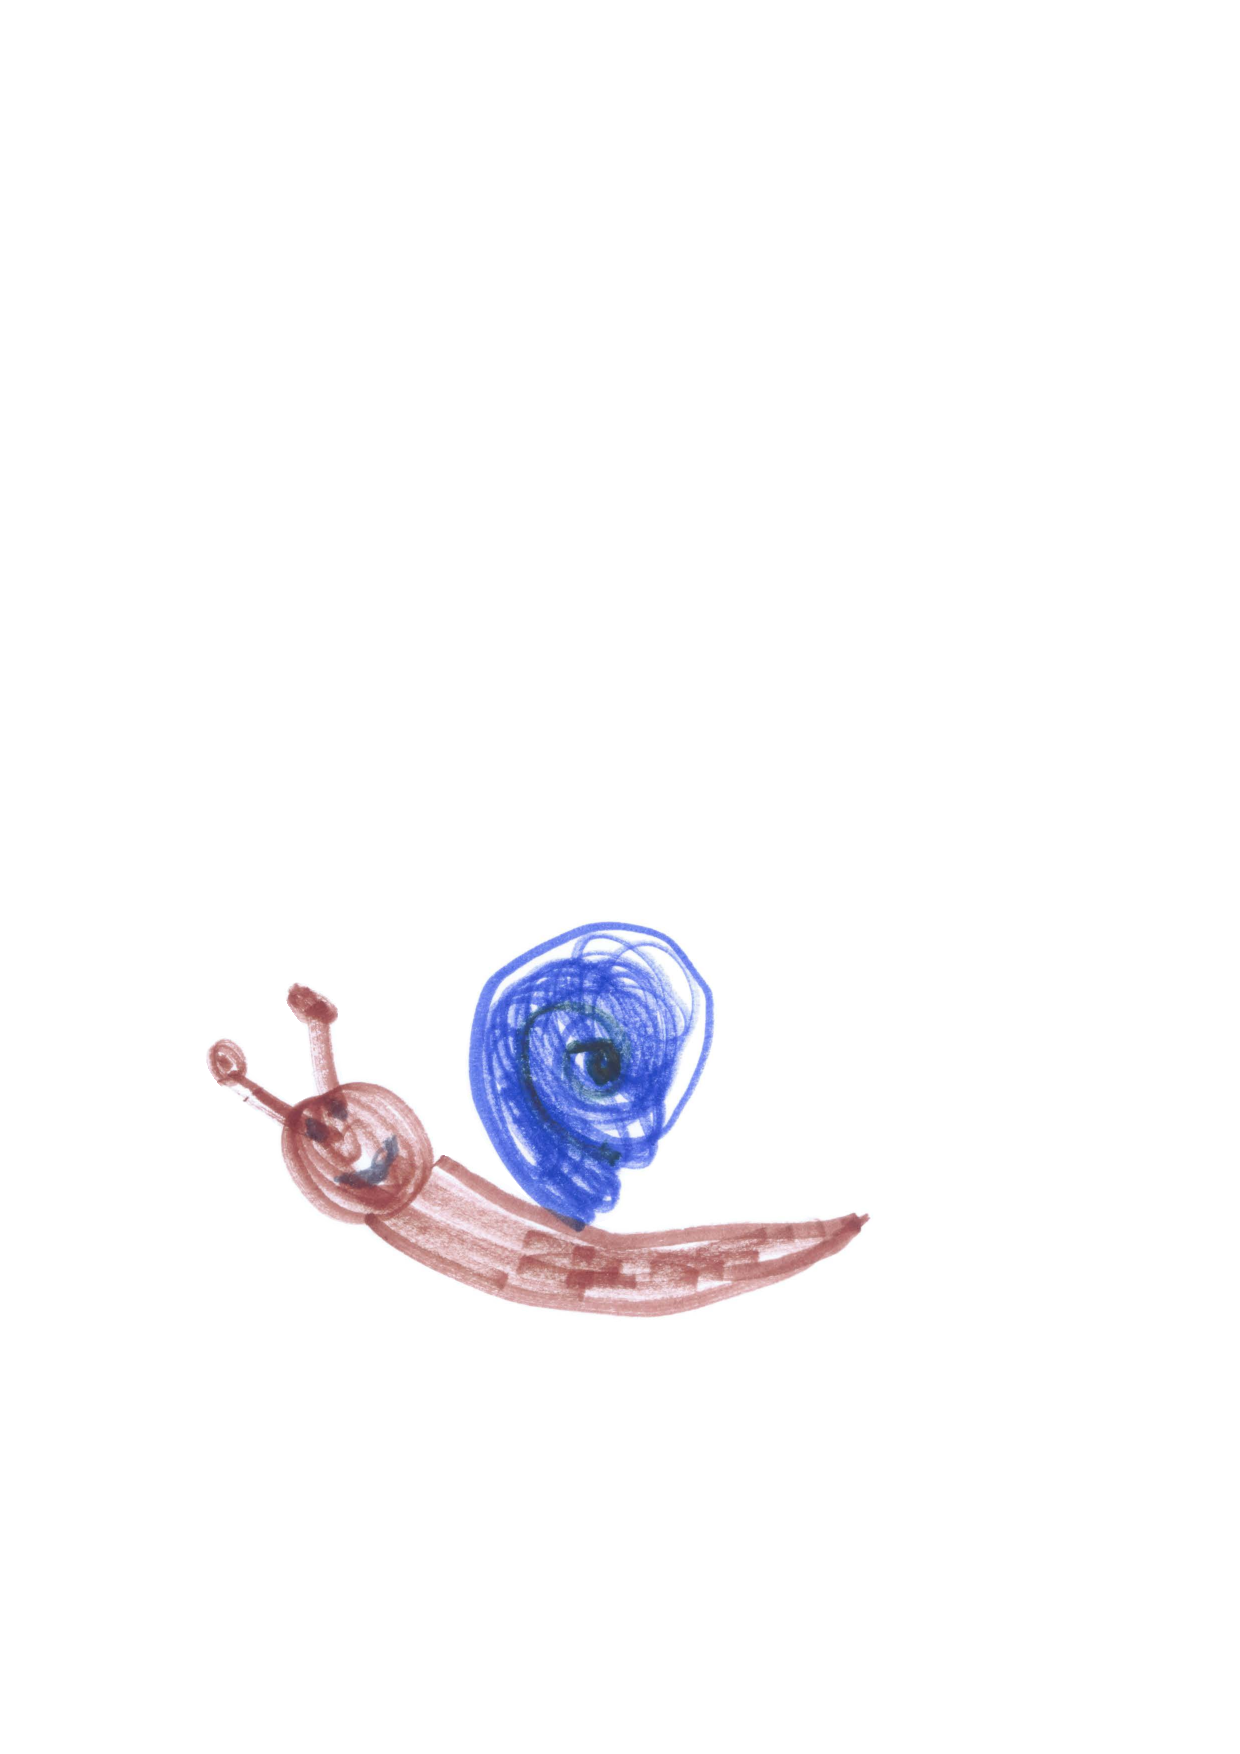
\includegraphics[width=\textwidth]{bilder/1schnecke.pdf}
    \end{figure}
    \clearpage
}

Aha, denkt Tabea Timpetampe. Eine sehr vornehme Schnecke. Gerade wie eine Prinzessin aus einem Märchen. Sie nimmt Herrn Häusler und setzt ihn in die Sandburg.

\enquote{Bitteschön!, Ihre eigene Burg.}, erklärt sie. Herr Häusler wird sichtbar grösser vor Stolz. Eine eigene Burg ist besser als Joggen, so viel wäre auch der dümmsten Schnecke klar gewesen. Sie spielen eine Weile zusammen. Herr Häusler ist die Prinzessin und Tabea Timpetampe die Baumeisterin. Herr Häusler lässt sich auch bereitwillig ein Kleid aus einem grossen Kastanienblatt basteln, in das er immer mal hinein beisst, wenn Tabea Timpetampe gerade nicht guckt. Vermutlich ist es ja unhöflich, ein Kleid, das man gerade bekommen hat, aufzuessen. Ganz sicher ist sich Herr Häusler auch nicht immer in Stilfragen.

Sie bauen noch eine Höhle und eine Strasse und verstecken einen Schatz in der Ecke des Sandkastens. Einen gestreiften Stein. Tabea Timpetampe ist zufällig grosse Expertin, wenn es um das Finden besonderer Steine geht. Im Wintergarten zwischen den Blumentöpfen liegt schon eine beachtliche Sammlung. Mama hat neulich sogar vorgeschlagen, dass Tabea Timpetampe alle Steine in einen echten Schuhkarton legen darf. Die weiss das also auch zu schätzen.

\enquote{Das ist jetzt unser Geheimnis.}, entscheidet Tabea Timpetampe und da kann Herr Häusler nur zustimmen. 

Ein grosses Weinen beginnt, denn Tabea Timpetampes Schwester ist umgefallen. Die Mama tupft an der Wunde herum und jetzt schnell nach Hause, heisst es. Tabea Timpetampe kann Mama gar nicht Herrn Häusler vorstellen, sie darf sich nicht einmal verabschieden. Sie wird -- zack -- von Mama am Arm genommen und ab geht es. So unbeachtet zu bleiben, gefällt Tabea Timpetampe überhaupt nicht, da weint sie lieber auch gleich mit.

Am nächsten Tag darf Tabea Timpetampe nicht im Sandkasten spielen, denn es regnet. Am Tag darauf werden die Grosseltern besucht und es ist noch irgendetwas, dass sie nicht so ganz genau verstanden hat. Aber es klappt wieder nicht, draussen zu spielen. Dabei hat sie doch so grosse Lust, Herrn Häusler wiederzusehen. 

Am Wochenende ist es endlich so weit. Aber Herr Häusler ist nicht mehr da. Natürlich nicht, so lange wartet ja niemand. Tabea Timpetampe ist sehr traurig und sucht überall. Vielleicht joggt er ja irgendwo auf der Wiese? Aber nichts. Weit und breit keine Schnecke. Bestimmt hat Herr Häusler sie längst vergessen. Sie mag gar nichts spielen.

Dann fällt Tabea Timpetampe der Schatz wieder ein. Sie sieht nach. Der Schatz ist noch da, aber es ist noch etwas dazu gekommen: ein Schneckenhaus, von Herrn Häusler, für sie. Da hat Tabea Timpetampe wieder Lust zu spielen. Sie baut die Burg wieder neu und die Strasse und die Höhle. Alles sogar noch ein bisschen grösser als das letzte Mal. Und sie vergräbt den Schatz neu, aber ohne das Schneckenhäuschen, das nimmt sie lieber mit nach Hause. \hfill {\color{DeepPink}\decofourleft}
